\section{Episode 71: Martin the Paranoid Android}

\medskip

\DndDropCapLine{D}ear Professor Mc’Caw,\medskip

As requested I am writing to inform you of my progress so far. My work placement found me travelling to Linderdorf with Mr (he insists of Professor and beats me if I either refuse or omit this honorific) Burnie and the rest of his, for want of a better word, crew. After a rather drawn out day of purchasing sausage meat stands and projectile vomiting, we had tried to track down a local famous blacksmith (I must admit I was a little starstruck) only to find out that they had been missing for sometime in the Varg. Professor Burnie and the crew agreed to help find these folks so I find myself heading to the Varg.\medskip

As we left, we met two dwarves (fine fellows indeed the dwarves, some of my best friends know dwarves) Linus Brandler, and Celina Speidel. They told us that they were in the employ of the workshop and were to join us on our quest. Riphard seemed tendacious and wanted to test the martial skills of our potential dwarven compatriots by throwing a lemon into the air and commanding that they fire. The lemon completed its arc and fell to the floor to the modest embarrassment of everybody there.\medskip

We set off Northwards in the fine sky boat, following the rough trail that we were made aware of back at the office. Two days passed with no incident at all. I spent my time making Pieces of Shit for Myron and trying to catch up on some of my assassin studies. One morning I awoke and as I took my morning exercise on deck, I notice that we had crossed the border into the snow-covered Varg Lands. My god, a splendid sight those rolling hills of plain white snow, the scattered small camps of nomadic underclasses. Intoxicating. Myron took point and cast out his eagle-eyed eyes over the barren wasteland, a true sight to behold this master of bushcraft, his keen sentry-ship being disturbed only by the occasional vomiting over the deck and the cry to refresh his drink. I did not have the heart to inform him that we were running low on Bovril.\medskip

We travelled for another day and a half. Far below we started to see roving bands of goblins and ogres, trompling along the landscape, no doubt enjoying the fine Winter that lay across the lands like the casual hand of a form tutor making its way onto the lap of an impressionable young boy who desperately needs that passing grade in his poison class. As I thrust my gaze over the landscape I noticed a set of tracks that looked unlike those we had seen before. I called over Myron and pointed out my find. I daresay I saw a glimpse of impressidness cross his craggy brow but one should keeps one’s egoism in check. Our dwarven companions seemed to agree with Myron’s assessment that these were the tracks we were looking for. I ducked out and went to milk Mrs Burnie, a task that fills me with equal parts dread and unknown excitement every day. I warmed two bottles and took them to Riphard. No-one seemed interested in this so I will not elaborate further.\medskip

Night fell. Professor tried to volunteer me for a suicide mission, a once-in-a-lifetime opportunity I’m led to believe. The sky boat pulled into a secluded spot and the professor and I disembarkened, Burnie covering the boat with a single branch in a masterful display of camouflage. We moved forwards with discretion, approaching the camp that we had seen from above. Aside from the usual goblins and horses, we spied three bearkin standing about a human garbered in rags, slouched down and enchained with long chains that somehow were propping him up against all natural laws of nature. On a second viewing I noticed the chains were actually holding him up, on account of being attached to local trees. The man kept regaining consciousness only to have it robbed from him again and again by the fists (paws) of the bearkin(g?). On a third viewing I noticed that the man’s face and most of his skin was in fact made of metal. From the notes I stole from Professor’s room I decided that this must be the kraftwerk mercenary Martin Andelberger. Professor decided we should attack ourselves but then he decided we should not. We went to fetch the remaining crew.\medskip

I stood watching, alone, surveying the fight to come. After a short time I heard the sounds of the rest of the crew coming towards us. So did a goblin and the battle was afoot. Riphard stepped forwards and flashed a million gold piece smile at the goblin and a nearby human. The goblin, halfway through attempting to howl, eased in his saddle and sent out something that seemed like a goblin greeting. Riphard nodded a gentle “be cool bro”. From across the expanse, the robot man stirred. A bearkin saw Riphard. Not good. A brief dialogue ensued but I could not make out the words. Myron ran in and just stood there in full view of everyone. I feared that Burnie had not communicated the plan very well. The confusion from our new goblin friends warmheartedness towards us seemed to be the only thing keeping them from attacking. They opened dialogue with Riphard who threw out the trading/investment spiel which worked so well when we fought the sausage vendor in Linderdorf. Apparently they had squandered some supplies from a sled, the very sled we had been tracking. The question came to me immediately. Where were the sled owners? A mystery. The merry band of mexican/new yorker Varg folk were having their fun with the brutalisation of the metal man. The varg folk told us that the sled owners had run off and that they were trying to squander what they could from the possessions they had left behind. I took the opportunity to light a horse’s testicles on fire, as per the professor’s instructions. The horses bolted into the snowy night. The bearking was not happy and ordered the goblin to round them up. Myron told him with the straightest face I have ever seen that there were strong pickings to the south. We seemed to have established a friendship, a brief glow of warmth in the icy, cold wasteland.\medskip

The Varg-Kin went South to find their fortune and we were left in possession of their beaten prisoner. Myron managed to wake up the robot man after about twenty minutes. He tried to talk to him about life but he was not enthusiastic about it. Myron gave him the footnotes about why we were here, which appeared to be both incomplete and written in another language. Martin claimed to have been the only one travelling and to have been here alone for years. Myron used the word “obvs” which I believe is short for oblivious. I implored the Professor to ask the robot if he could be of any use to us. Martin said something so cutting, so unbelievably devastating that Burnie visibly winced and started also to cry a little bit. I asked him if he was indeed a companion of Grunhelvem and Indelnacht. He cryptically said yes and started sledding away, yet we dastardly jumped onto the sled. I told him we had need of his knowledge to help in the task that I still do not understand. Riphard told him we required their knowledge to craft weapons of excalibrum. Martin did not seem to know what this is. I spent some time trying to convince Mr Martin to help us re-pick up the trail of our quarry, and asking about his purpose in life. Suddenly, the sky boat appeared above and a giant cable with a hook fell out of the bottom hole, which picked up Martin by his buttocks. However, the robot man did not rise, rather the boat fell towards him. I pleaded one more time for his help but he refused and set off on his way. I left it a moment and then covered my face in snow and followed directly in his footsteps. After only five minutes I noticed that his gaze had been directed to a new set of tracks and he diverted his path to follow them. The airship followed at some distance. Someone had decided to engorge the ship in a cloud of brown gas which, if anything, only added to the conspicuousness of the dirigible.\medskip

Hours passed. Martin was slow. I took the opportunity to have a short nap. But it was too cold to sleep and the only outcome was that I ended up with a, what I suspect was a piss stained, blanket frozen onto my lower body. I decided that it would make more sense to simply ask if I could sit on the sled and Martin was kind enough to acquisition. I pointed out to Martin that the Varg was in the other direction. He paused and produced a small bedroll. We spent some time talking. He said he couldn’t die which seemed excessive. We chatted university. We chatted the past. He kept stuttering. And then he crashed. I am confused. We started to load him onto the ship through the claw mechanism. I thought that perhaps I was next but instead the claw came down and took the bedroll from me. Professor suggested it was better for me to stay on the ground, sharpen the senses and take point. I tried to argue but I’m learning that you cannot argue against a man such as Burnie. With a sigh, I picked up the rope and continued dragging the broken sled along, following the tracks that Martin had located. They took my woolen top hat with the claw.\medskip

From what I gather, whilst I was down below, the remaining crew were taking it upon themselves to try and fix Martin’s stutter. Apparently a quick shock from the Professors glove did the trick. Burnie made love to a bird man apparently. Some harsh words followed directed at Myron. But Myron persisted in his questioning. Martin was created in Linderdorf. That was all that was learned before I collapsed.\medskip

I’m told that Martin had jumped over the side to rescue me. Professor says that he then used a quote “cable hand” to hoist us both back onto the skyship. Myron took over the role of track following from the comfort and warmth of the sky boat. So brave. I feel so foolish that had the nerve to be so weak and collapsed in the sub zero temperatures. Myron called Martin’s bluff and tried to steer North towards the Varg, a clever ruse to gain more information from our new prisoner/guest/travelling companion. Adding to the disaster of the lie was the fact that our new dwarf companions recognised Martin. They revealed that Martin had been an official member of the party going North. Martin tried to jump off the boat again but was stopped. The dwarves made the point that the other travellers would be a week or so ahead. I woke up to find Myron standing over me screaming Bovril. Oh god. I crawled over to the bar and checked the Bovril box. I can’t describe the feeling that came over me as I stared into that dark, empty box. I looked at Myron. Myron looked at me. A bead of sweat ran down my face. “Is there a problem boy?” he asked, fingers itching towards his abomination of a gun sword thing. I tried to put on my best smile and started pouring in the grenadine. I dropped a bottle of sherry but we had more. Then it came to the last ingredient. I looked at Myron again and smiled. He was not smiling. I looked around desperately and then I saw it. A chance. A small carton of instant gravy. Did I dare? How could I not. I slowly stirred a spoonful of those delicate meaty granules. It seemed to take almost an eternity for them to dissolve in the tepid liquid but finally it was done. With shaking hands, I handed the glass to Myron. I held my breath as he raised the glass to his lips and sipped deeply. Time stopped. Would he know, would he see through my ruse? How could he not? But then a miracle. For the first time in this last month, I saw something that looked like a smile cross his face. A miracle.\medskip

As the days went on the weather closed in. Myron (possibly) joked that they would need me on the ground again to follow the tracks. I’d only just got the feeling back in my fingers. It seemed to be a snow storm although it was the oddest thing, the air seemed to be closer, pressured. Myron and Martin looked troubled, whatever that means on a robot’s face. We tried to push on through the evening but as time went on the winds got stronger, the colour of the storm became deeper, the temperature cooler. We felt a strong shock to the sky boat which knocked us to the floor. Suddenly, there was a gigantic crack and the air became electric as a lightning bolt hit the sky boat. The last thing I saw was the mountain and the very large footsteps that crossed over the trail we were following...\medskip

Yours sincerely,\medskip

Kevin J Eldon\medskip

\textbf{Epilogue}\medskip

“Dear Myron,\medskip

This is the third letter I’ve tried to write to you, but somhow i cant seem to find it in myself to send a singel one. I think im scared you wuldnt want to here from me. Ive been trying to mak up for sum of the things that hav hapened over the last few munths. I dont fink il ever reely be able to, but i fought to myself, i shuld try. Its strange not beeeing in fights evryday. My life theese last few weeks has been quiet quiet comapred to the last year or so. I fink youd like the slower life in a way. Maybee yuu wuould be a bit bored thouh bacaseu i know you like kiling monsters and fings.\medskip

I hope Burnies is looking affter you. I hope yure not drinking tooo much.\medskip

I think about delilah every day. I see her in my nitemares every nite, a thousand times i hear her screams and watch her make eye contact with me before reachinng out to her childern wiht her last action. Sometimes i fhink about the way you looked at mee that last time…”\medskip

Exmerah put her pen down and looked down at the piece of parchment that lay in front of her. She sat there staring at it for a long time...\medskip

https://www.youtube.com/watch?v=wZdZKolMIl0

\vspace*{5mm}

\begin{center}
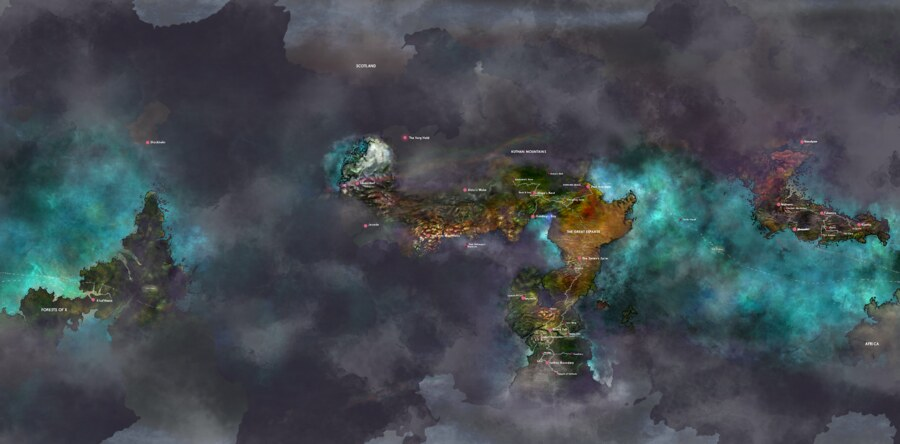
\includegraphics[width=\textwidth]{./content/img/velterraMap.jpg}
\begin{figure}[h]
\end{figure}
\end{center}

\clearpage
